\documentclass[10pt]{article}

\usepackage{spheric}
%%%TITLE
\title{Interaction between Solitary Wave and Flexible Plate based on MPS-FEM coupled Method}
\date{}

%%AFFILIATIONS
\author[$\relax$]{Chengping Rao}
\author[$\relax$]{Decheng Wan$^\dagger$}
\affil[$\relax$]{State Key Laboratory of Ocean Engineering, School of Naval Architecture, Ocean and Civil Engineering, Shanghai Jiao Tong University, Collaborative Innovation Center for Advanced Ship and Deep-Sea Exploration, Shanghai 200240, China}
\affil[$\relax$]{\email{\dagger}{dcwan@sjtu.edu.cn}}


%%DOCUMENT
\begin{document}

\maketitle

%\SelectedTopics{}

%%PLEASE PUT YOUR ABSTRACT HERE
\begin{abstract}
The model of wave interacting with the plate is commonly seen in the offshore and coastal engineering. For example, a very large floating structure (VLFS) with its horizontal size much greater than the vertical size is usually treated as thin plate floating in the ocean. While encountering severe wave, it could produce considerable deformation which will exert a great influence on the flow field nearby, making the problem more complex. To conduct the FSI analysis of the wave-plate interaction problem, the Moving Particle Semi-Implicit and finite element coupled method (MPS-FEM) is proposed. The MPS method is adopted to calculate the fluid domain while the structural domain is solved through FEM method.

The solitary wave is first generated in a numerical wave tank and then be compared with the theoretical wave profile. The convergence study with regard to particle resolution is conducted to find the appropriate particle spacing employed in the following simulations. Then the simulations of various solitary wave impacting onto flexible plate are conducted. To validate the accuracy of the current FSI solver, the wave-induced force on the plate is compared with the existent experimental result, which shows a good agreement. The effects of the structural deformation on the flow is investigated. It turns out that the vibration of the flexible plate may intensify the impact with the free surface. In addition, the maximum displacement on the middle-point of the plate under wave with various amplitude is collected to examine quantitatively the structural response to the impact.

\begin{figure}[!htb]
\begin{minipage}[b]{0.33\linewidth}
\centering
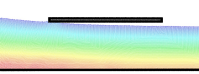
\includegraphics[width=\textwidth]{17-11.png}\\
(a)
\end{minipage}
\begin{minipage}[b]{0.33\linewidth}
\centering
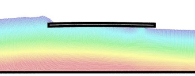
\includegraphics[width=\textwidth]{17-12.png}\\
(b)
\end{minipage}
\begin{minipage}[b]{0.33\linewidth}
\centering
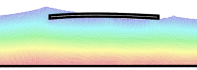
\includegraphics[width=\textwidth]{17-13.png}\\
(c)
\end{minipage}

\begin{minipage}[b]{0.33\linewidth}
\centering
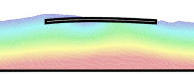
\includegraphics[width=\textwidth]{17-14.png}\\
(d)
\end{minipage}
\begin{minipage}[b]{0.33\linewidth}
\centering
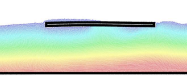
\includegraphics[width=\textwidth]{17-15.png}\\
(e)
\end{minipage}
\begin{minipage}[b]{0.33\linewidth}
\centering
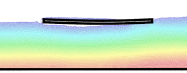
\includegraphics[width=\textwidth]{17-16.png}\\
(f)
\end{minipage}
\caption{Snapshots of the wave-plate interaction}\label{fig:17-1}
\end{figure}

\end{abstract}


%%THE END OF ABSTRACT

%\addbib

\end{document}
